\section*{Reflexión total interna}

\item A través de dibujos verifique que:
\begin{enumerate}
	\item Un rayo que incide sobre una lámina de caras paralelas, inmersa en un medio único, no se desvía al atravesarla. Calcule el desplazamiento lateral de dicho rayo, en términos de su espesor $d$ y de su índice de refracción $n$.
	\item El rayo que se refleja en la primera cara y el que emerge luego de reflejarse en la segunda son paralelos.
\end{enumerate}
Si el medio exterior es único, ¿existe algún ángulo de incidencia tal que produzca reflexión total en la cara inferior?



\item (*)
\begin{minipage}[t][3.5cm]{0.75\textwidth}
Un rayo incide con ángulo $\phi$ sobre la superficie horizontal de un cubo de material transparente, de índice $n$, inmerso en aire.
\begin{enumerate}
	\item ¿Para qué valores de $\phi$ hay reflexión total en la cara vertical?
	\item Si $\phi=60^{\circ}$, ¿cuál es el máximo $n$ para que no haya reflexión total en la cara vertical?
	¿Se puede reflejar totalmente en la cara superior?
\end{enumerate}
\end{minipage}
\begin{minipage}[c][1.5cm][t]{0.15\textwidth}
	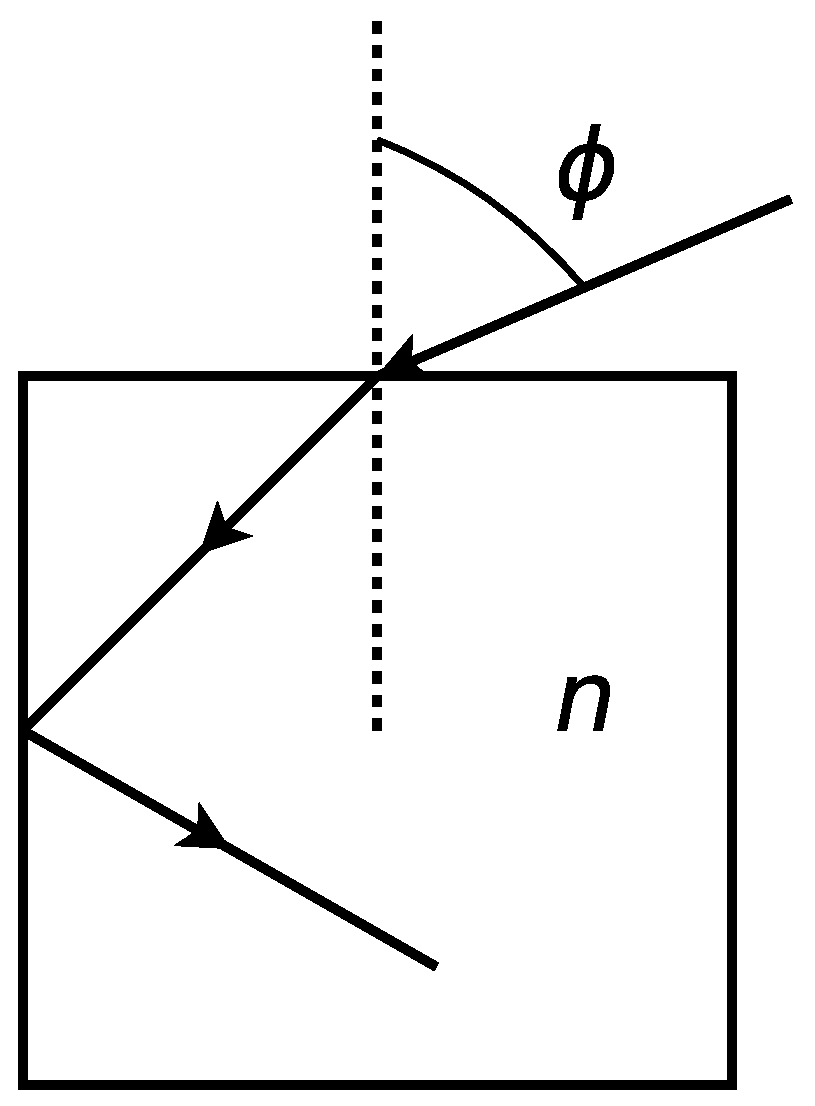
\includegraphics[width=\textwidth]{ej3-5}
\end{minipage}



\item
La fibra óptica es un medio empleado habitualmente para la transmisión de redes de datos, que se usa en telecomunicaciones.
Básicamente consiste en una hebra muy fina de cierto vidrio (cristal de silicio o materiales plásticos adecuados), de alto índice de refracción (núcleo), cuyo diámetro no excede los \SI{125}{\micro\metre}, que se recubre con un material de índice de refracción menor que el del propio núcleo (recubrimiento) con el fin de retener la luz dentro de él, y, que a su vez se protege con una envoltura exterior de material plástico muy flexible.
El funcionamiento de estas fibras está basado en el fenómeno de reflexión total sobre los rayos que, ingresando en un extremo, se reflejan sobre las paredes de separación entre el núcleo y el recubrimiento quedando así encapsulados hasta salir por el otro extremo, independientemente que la fibra siga o no una línea recta.
\begin{figure}[ht]
	\centering{}\includegraphics[width=0.75\textwidth]{fibra}
\end{figure}
\begin{enumerate}
	\item Demuestre que el ángulo del cono de aceptación \(\alpha_A\) que forman todos los rayos que ingresando en la fibra, como está indicado en la figura, son reflejados en la superficie de separación entre el núcleo y su recubrimiento es
	\[
		\sen{(\alpha_A)} = \frac{n_1}{n_o} \sqrt{1- \left( \frac{n_2}{n_1} \right)^2 }
	\]
	siendo \(n_0\) , \(n_1\) y \(n_2\) los índices de refracción que corresponden al medio exterior, al núcleo de la fibra óptica y a su recubrimiento, respectivamente.
	\item Como el cono de aceptación depende del índice que rodea a la fibra en el extremo de entrada, suele emplearse una magnitud denominada apertura numérica y que se define como
	\[
		\text{AN} = n \sen{(\alpha_A)}
	\]
	Calcule la apertura numérica correspondiente a una fibra cuyo núcleo tiene un índice de refracción de \num{1.66} y el correspondiente a su recubrimiento es \num{1.4}.
	Para estos valores, ¿cuál es el ángulo de aceptación si la luz proviene del aire? ¿Y si proviene del agua?
	\item ¿Qué rango de valores debería tener el índice de refracción del recubrimiento de un núcleo cuyo índice es \num{1.66} para que todo rayo que incida desde el aire quede atrapado dentro de la fibra?
\end{enumerate}



\item Los índices de refracción de cierta clase de vidrio para el rojo y el violeta valen: $1.51$ y $1.53$; respectivamente.
Halle los ángulos límites de reflexión total para rayos que incidan en la superficie de separación vidrio-aire.
¿Qué ocurre si un rayo de luz blanca incide formando un ángulo de 41$^{\circ}$ sobre dicha superficie?
